\section{Extra results}\label{annexe:extra_results}

In this appendix, we present some extra results that are of interest in order to demonstrate the performances of our method and algorithm.

\subsection{Simulated data}\label{annexe:extra_results_simulated}

TODO: des données qui ne ressemblent pas du tout à des données M/EEG.

\begin{figure}[h!]
    \centering
    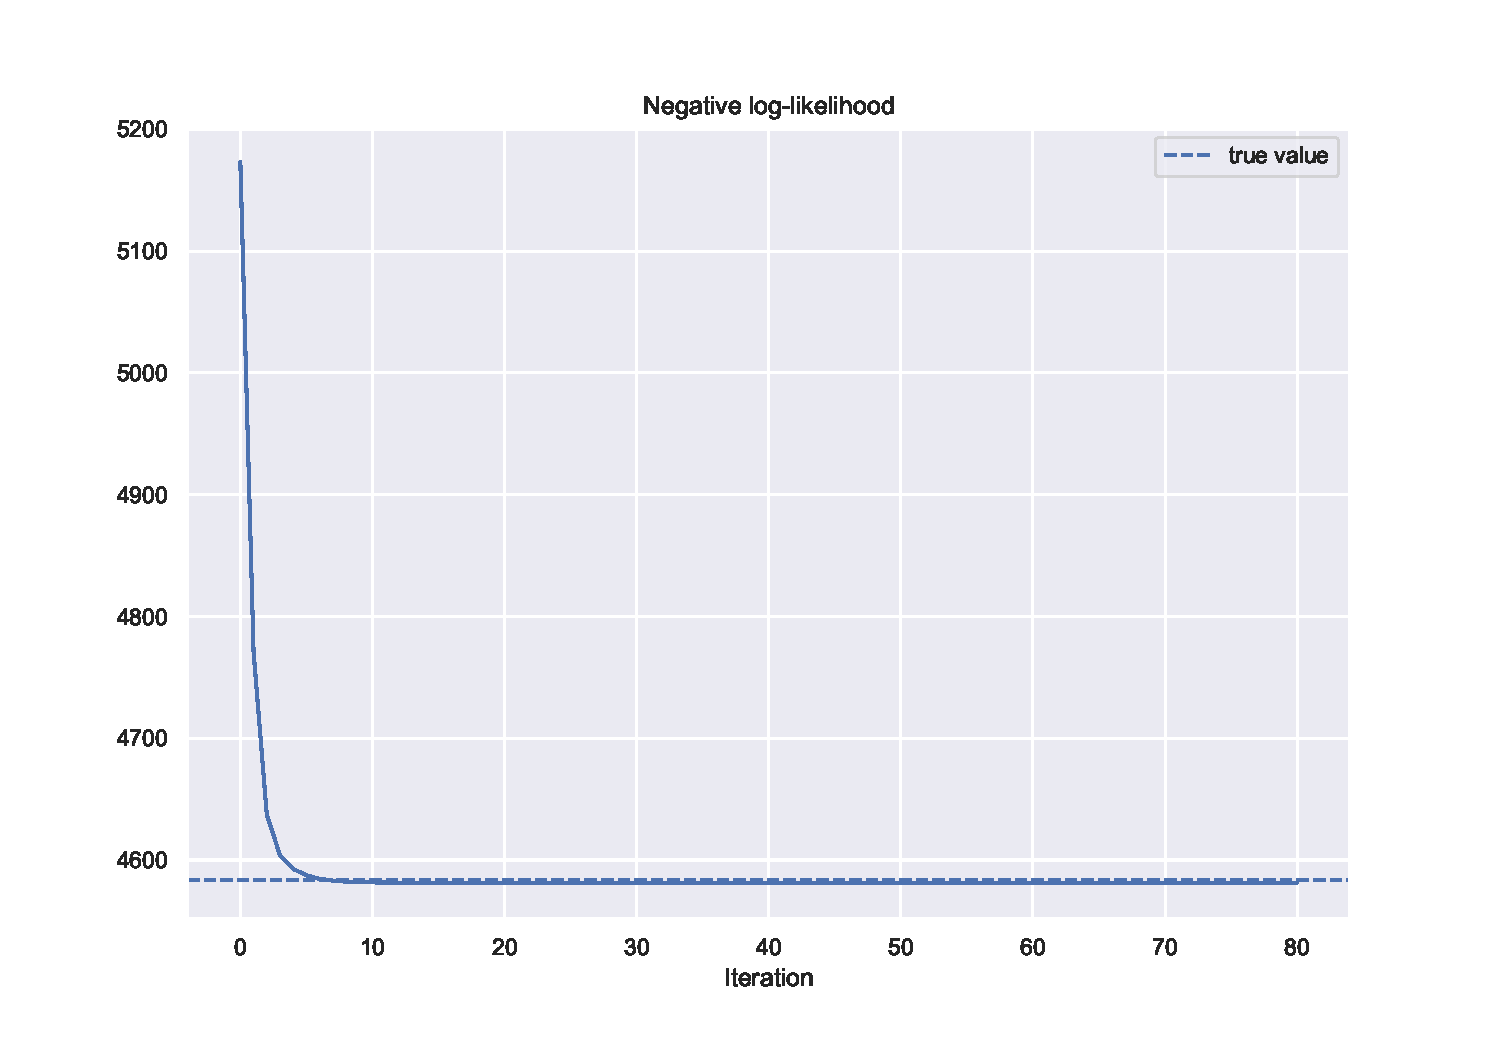
\includegraphics[width=0.9\textwidth]{pics/results/history_loss_2.pdf}
    \caption{Loss history over 80 iterations with a \textit{smart} initialisation, on simulated data with $T = \SI{100}{\minute}$, $\texttt{isi}=\SI{5}{\second}$, $\texttt{n\_tasks} = \SI{50}{\percent}$, $\intervalleFF{a}{b} = \intervalleFF{0}{2000}\times \SI{e-3}{\second}$.}
    \label{fig:history_loss_2}
\end{figure}

\begin{figure}[h!]
    \centering
    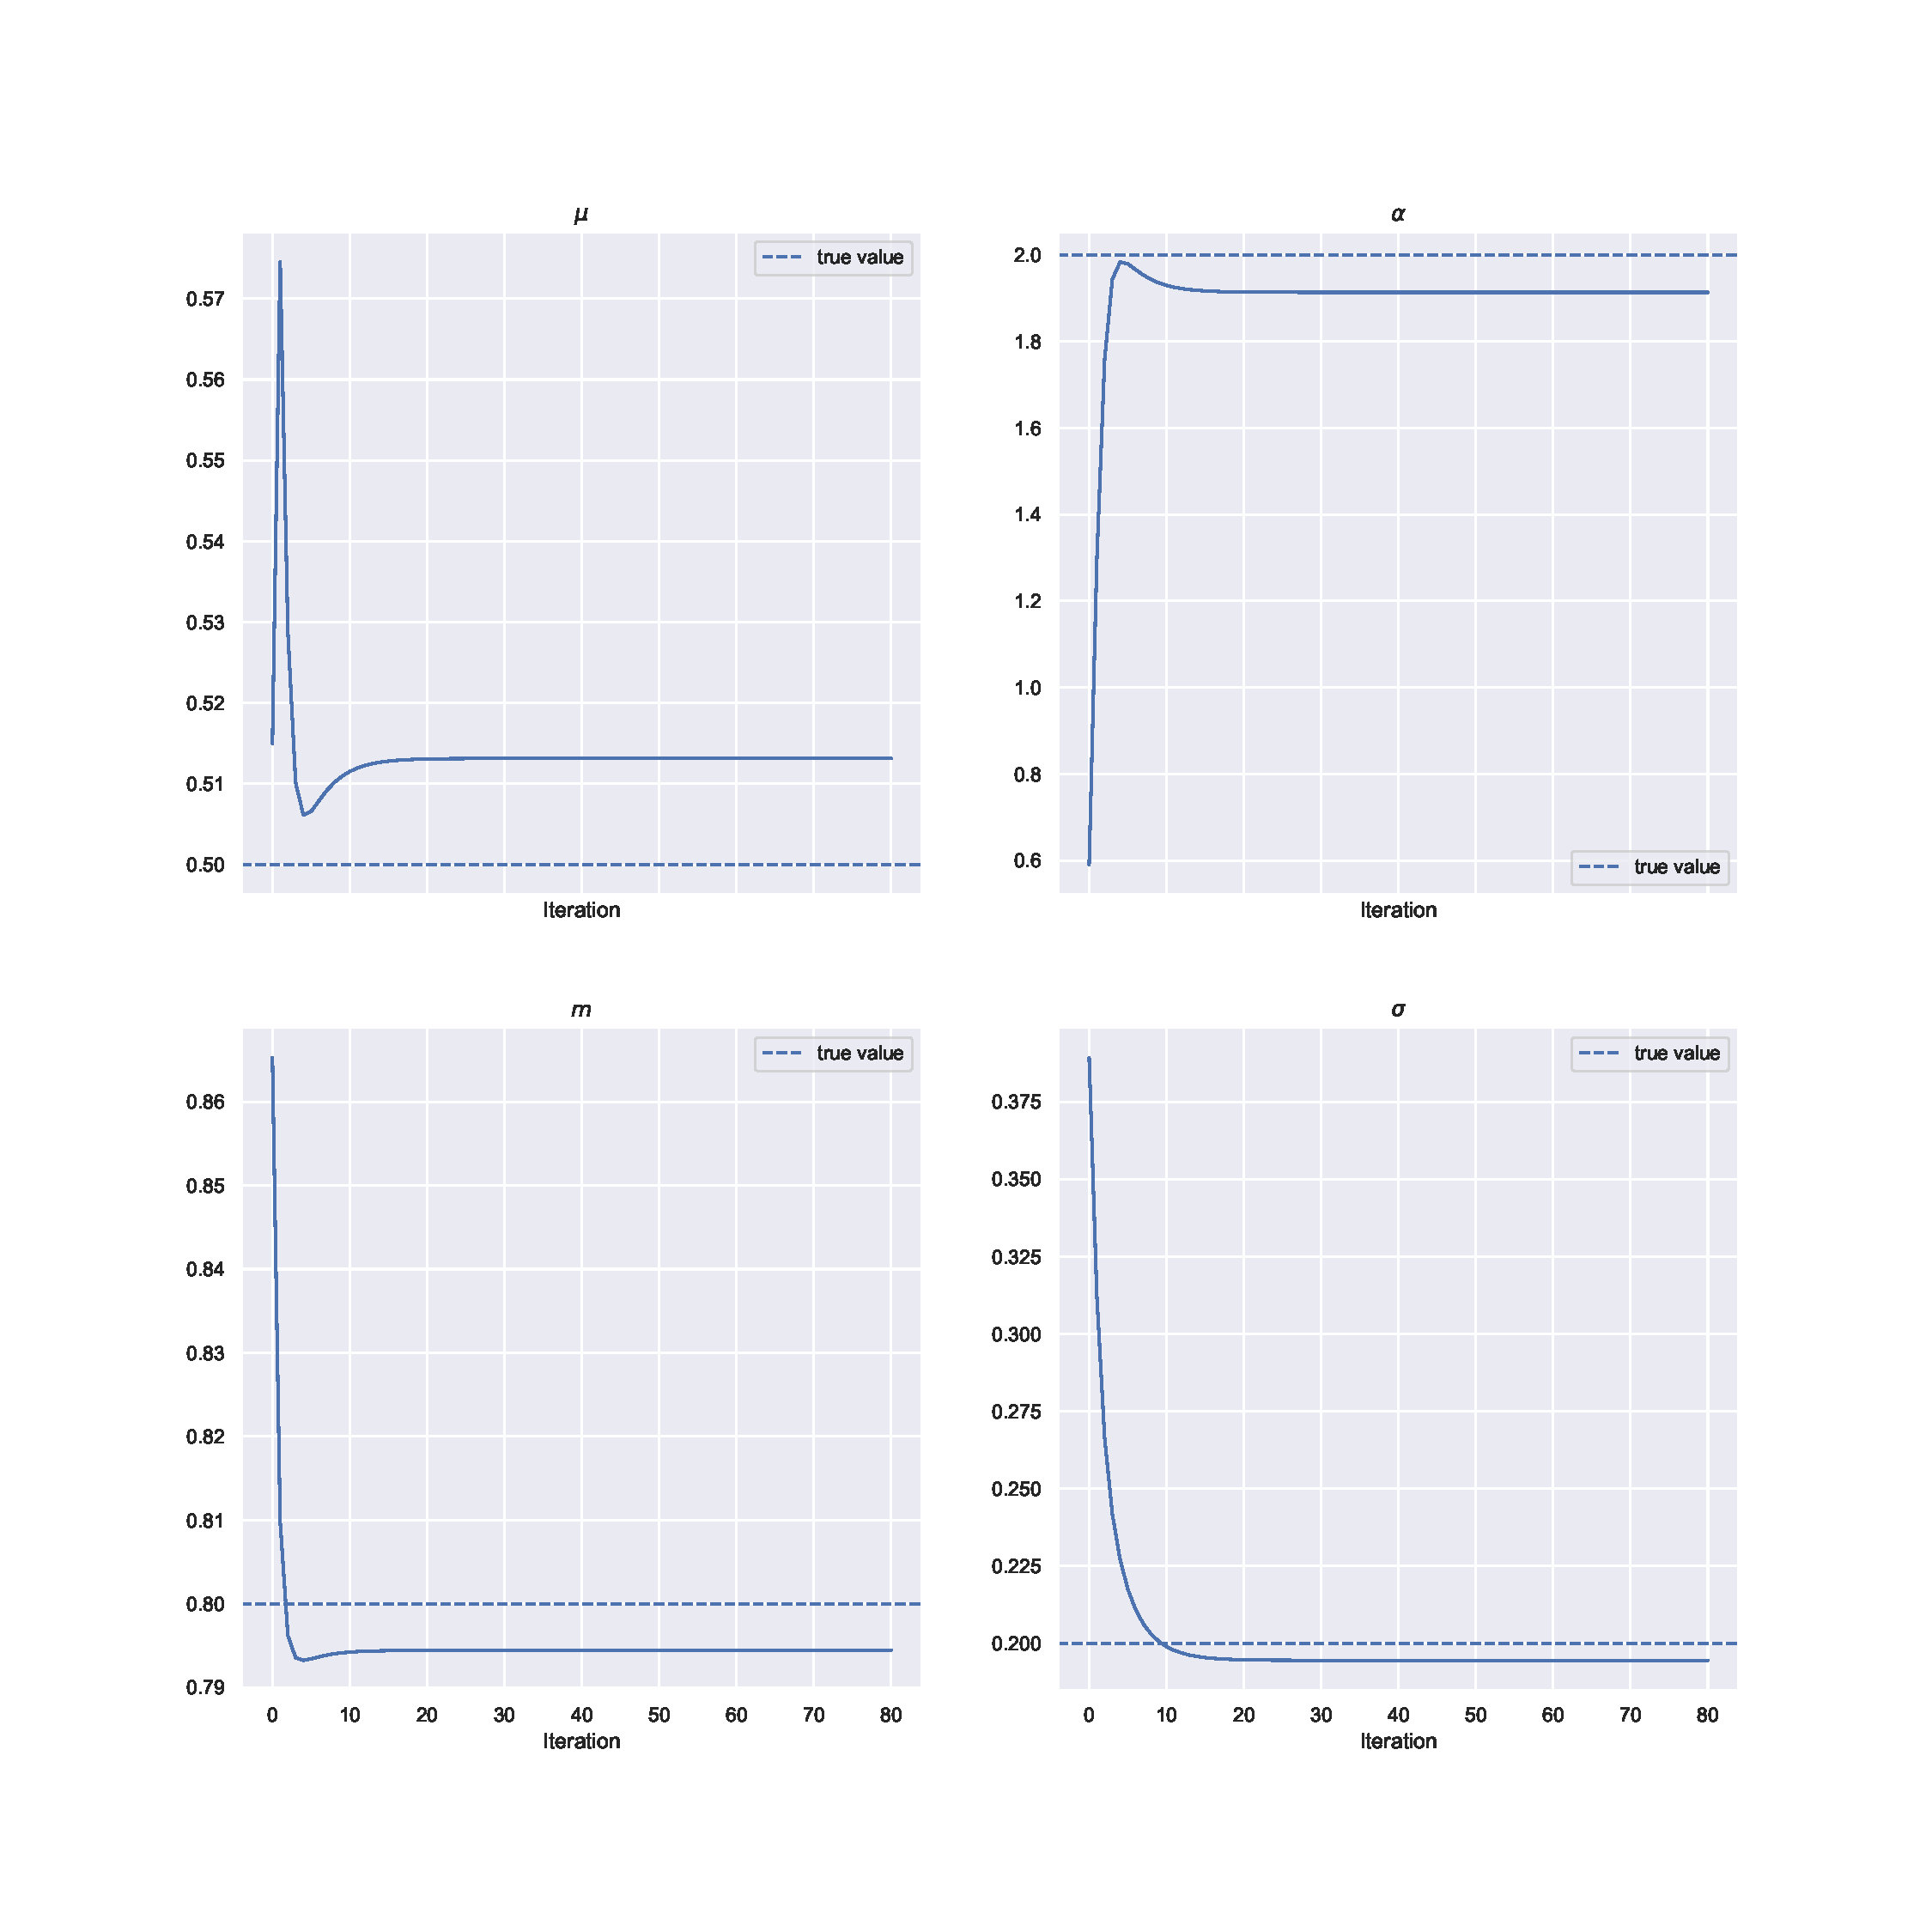
\includegraphics[width=\textwidth]{pics/results/history_params_2.pdf}
    \caption{Parameters recovery over 80 iterations with a \textit{smart} initialisation, on simulated data with $T = \SI{100}{\minute}$, $\texttt{isi}=\SI{5}{\second}$, $\texttt{n\_tasks} = \SI{50}{\percent}$, $\intervalleFF{a}{b} = \intervalleFF{0}{2000}\times \SI{e-3}{\second}$.}
    \label{fig:history_params_2}
\end{figure}

TODO: des données très similaires aux données réelles utilisées (\textit{sample}).
Note that in order to simulate data as similar as the \textit{sample} data, the hyper-parameter \texttt{n\_tasks} is no longer a percentage, but directly an integer, denoting the exact number of tasks timestamps we want to keep.

\begin{figure}[h!]
    \centering
    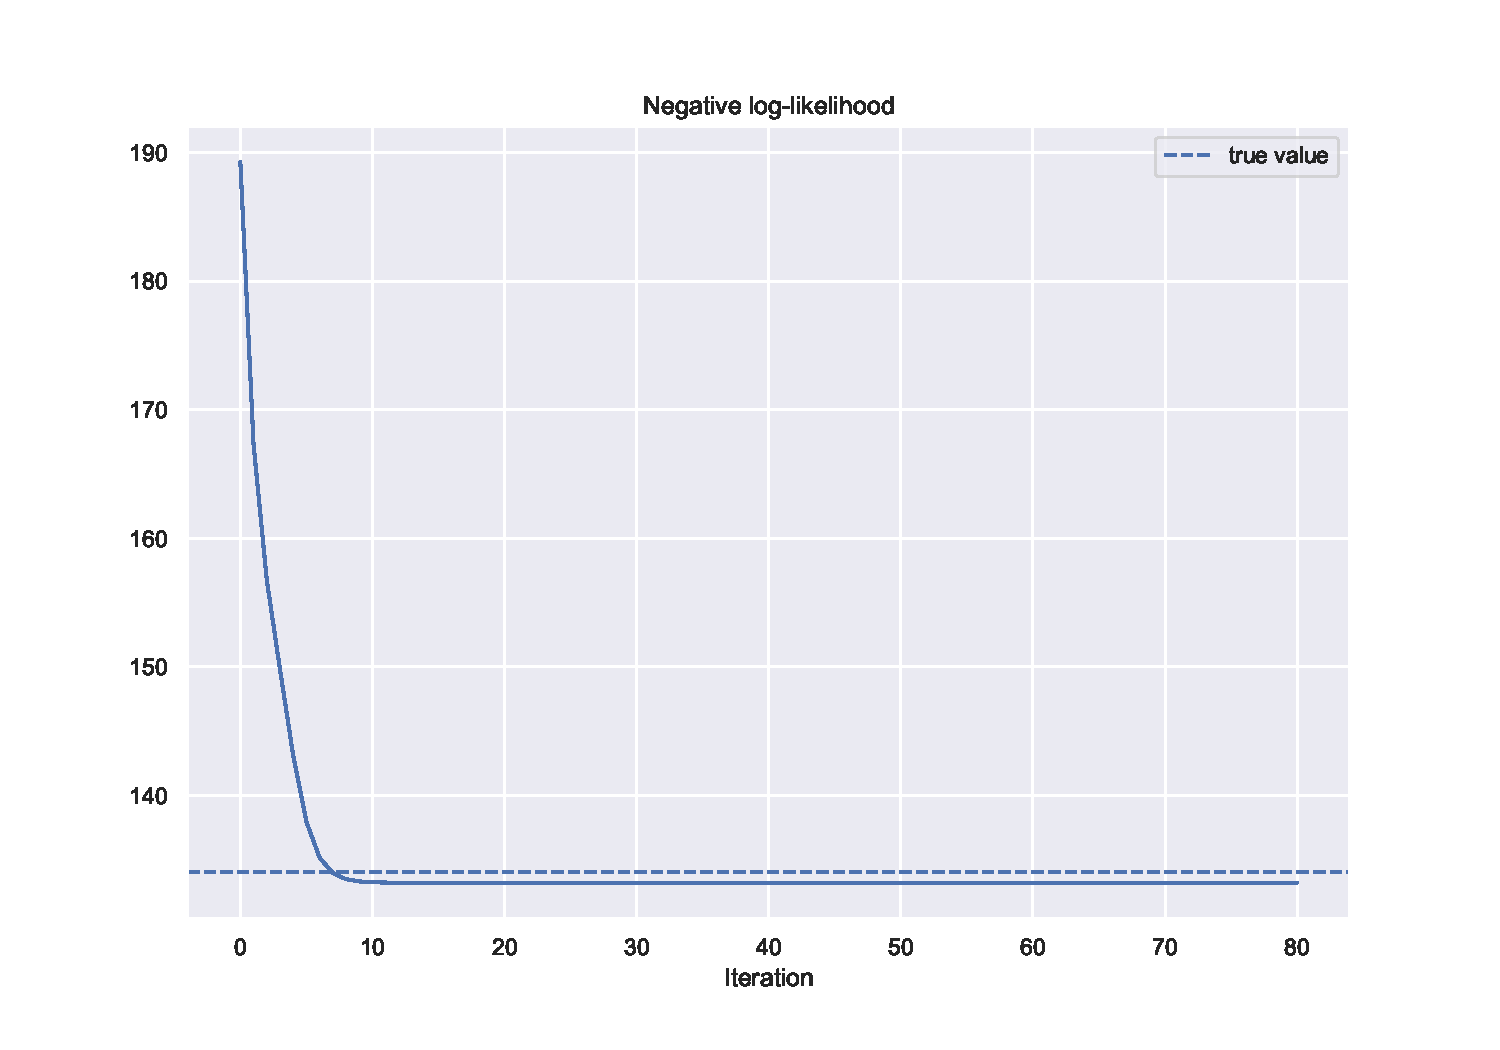
\includegraphics[width=0.9\textwidth]{pics/results/history_loss_simu_sample.pdf}
    \caption{Loss history over 80 iterations with a \textit{smart} initialisation, on simulated data with $T = \SI{4.6}{\minute}$, $\texttt{isi}=\SI{2.5}{\second}$, $\texttt{n\_tasks} = 70$, $\intervalleFF{a}{b} = \intervalleFF{30}{800}\times \SI{e-3}{\second}$.}
    \label{fig:history_loss_2}
\end{figure}

\begin{figure}[h!]
    \centering
    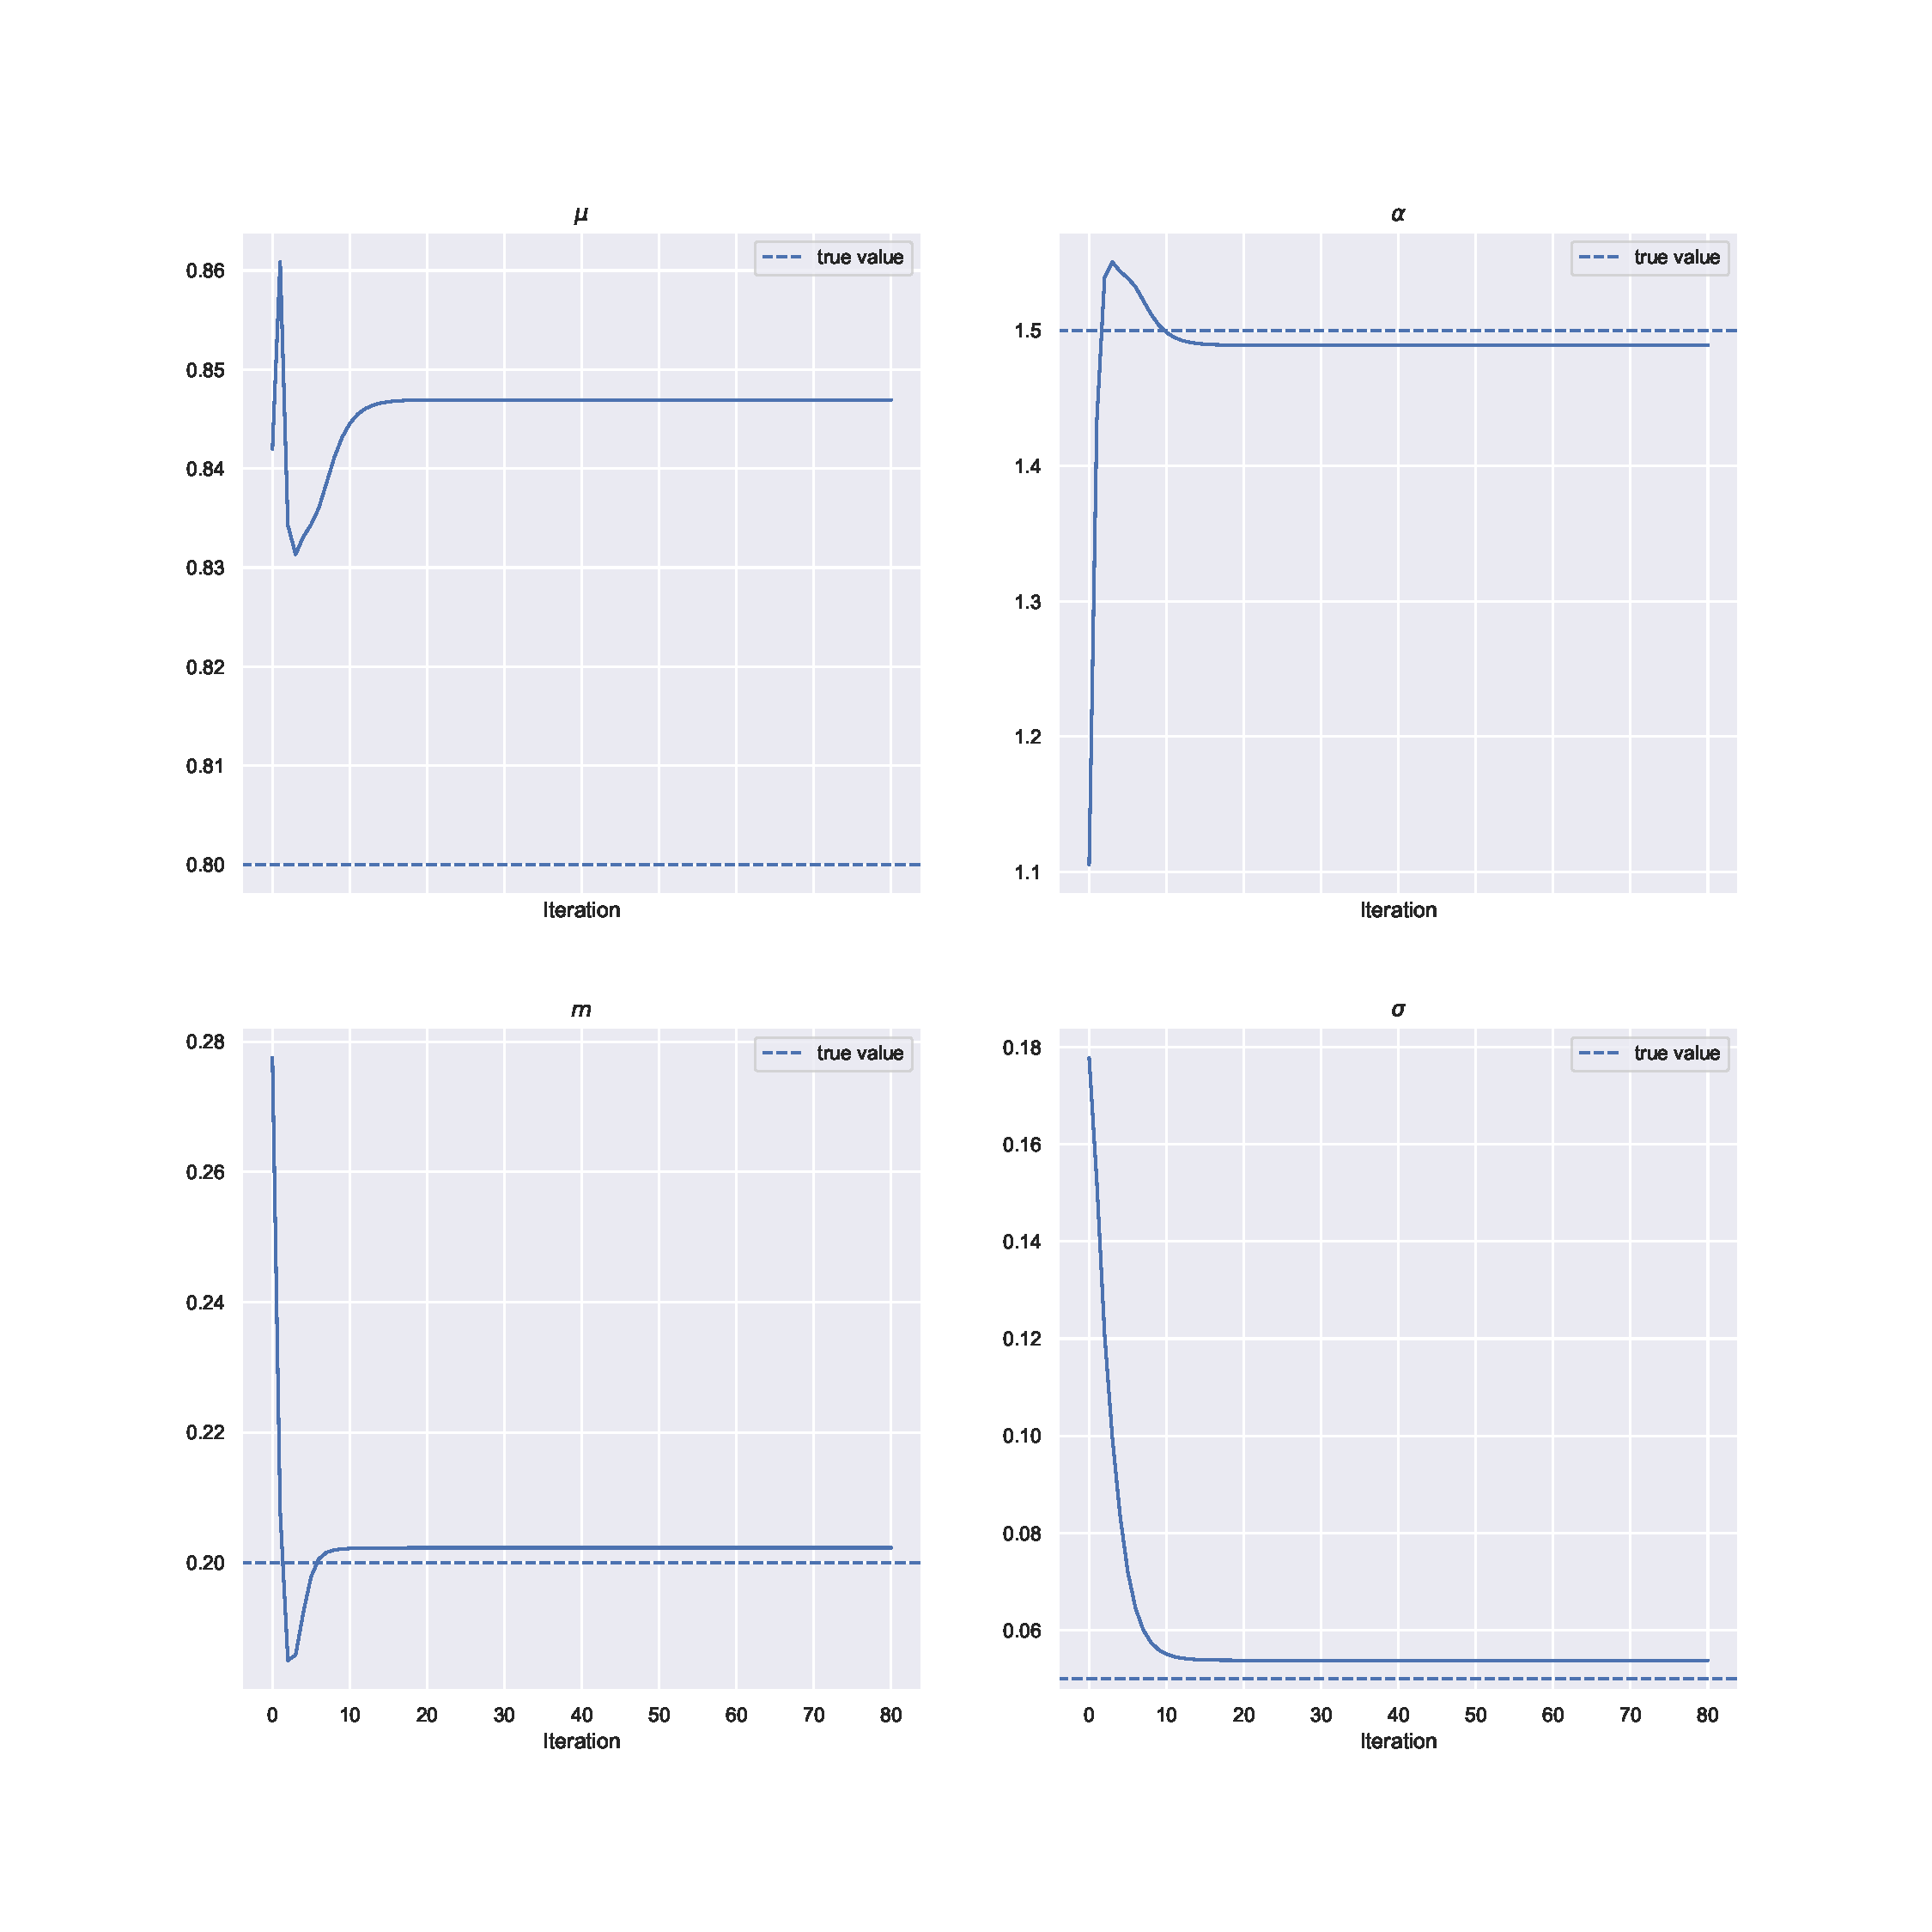
\includegraphics[width=\textwidth]{pics/results/history_params_simu_sample.pdf}
    \caption{Parameters recovery over 80 iterations with a \textit{smart} initialisation, on simulated data with $T = \SI{4.6}{\minute}$, $\texttt{isi}=\SI{2.5}{\second}$, $\texttt{n\_tasks} = 70$, $\intervalleFF{a}{b} = \intervalleFF{30}{800}\times \SI{e-3}{\second}$.}
    \label{fig:history_params_2}
\end{figure}

\subsection{Real data}\label{annexe:extra_results_real}

Figures~\ref{fig:history_loss_atom_0_task_1_2_3_4} and~\ref{fig:history_params_atom_0_task_1_2_3_4} show respectively loss and parameter history for EM algorithm carried out on atom 0 alongside all considered stimuli.

\begin{figure}[h!]
    \centering
    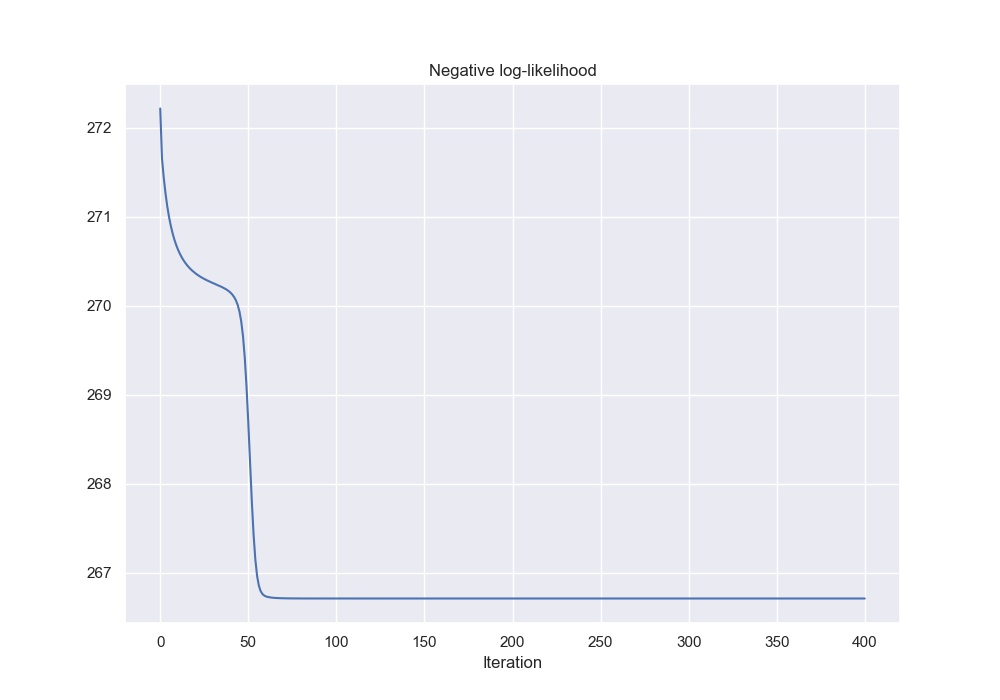
\includegraphics[width=0.9\textwidth]{pics/results_sample/history_loss_atom_0_task_1_2_3_4.jpg}
    \caption{Loss history over 400 iterations with a \textit{smart} initialisation, on sample data (atom 0, task 1, 2, 3 and 4) with $\intervalleFF{a}{b} = \intervalleFF{30}{800}\times \SI{e-3}{\second}$.}
    \label{fig:history_loss_atom_0_task_1_2_3_4}
\end{figure}

\begin{figure}[h!]
    \centering
    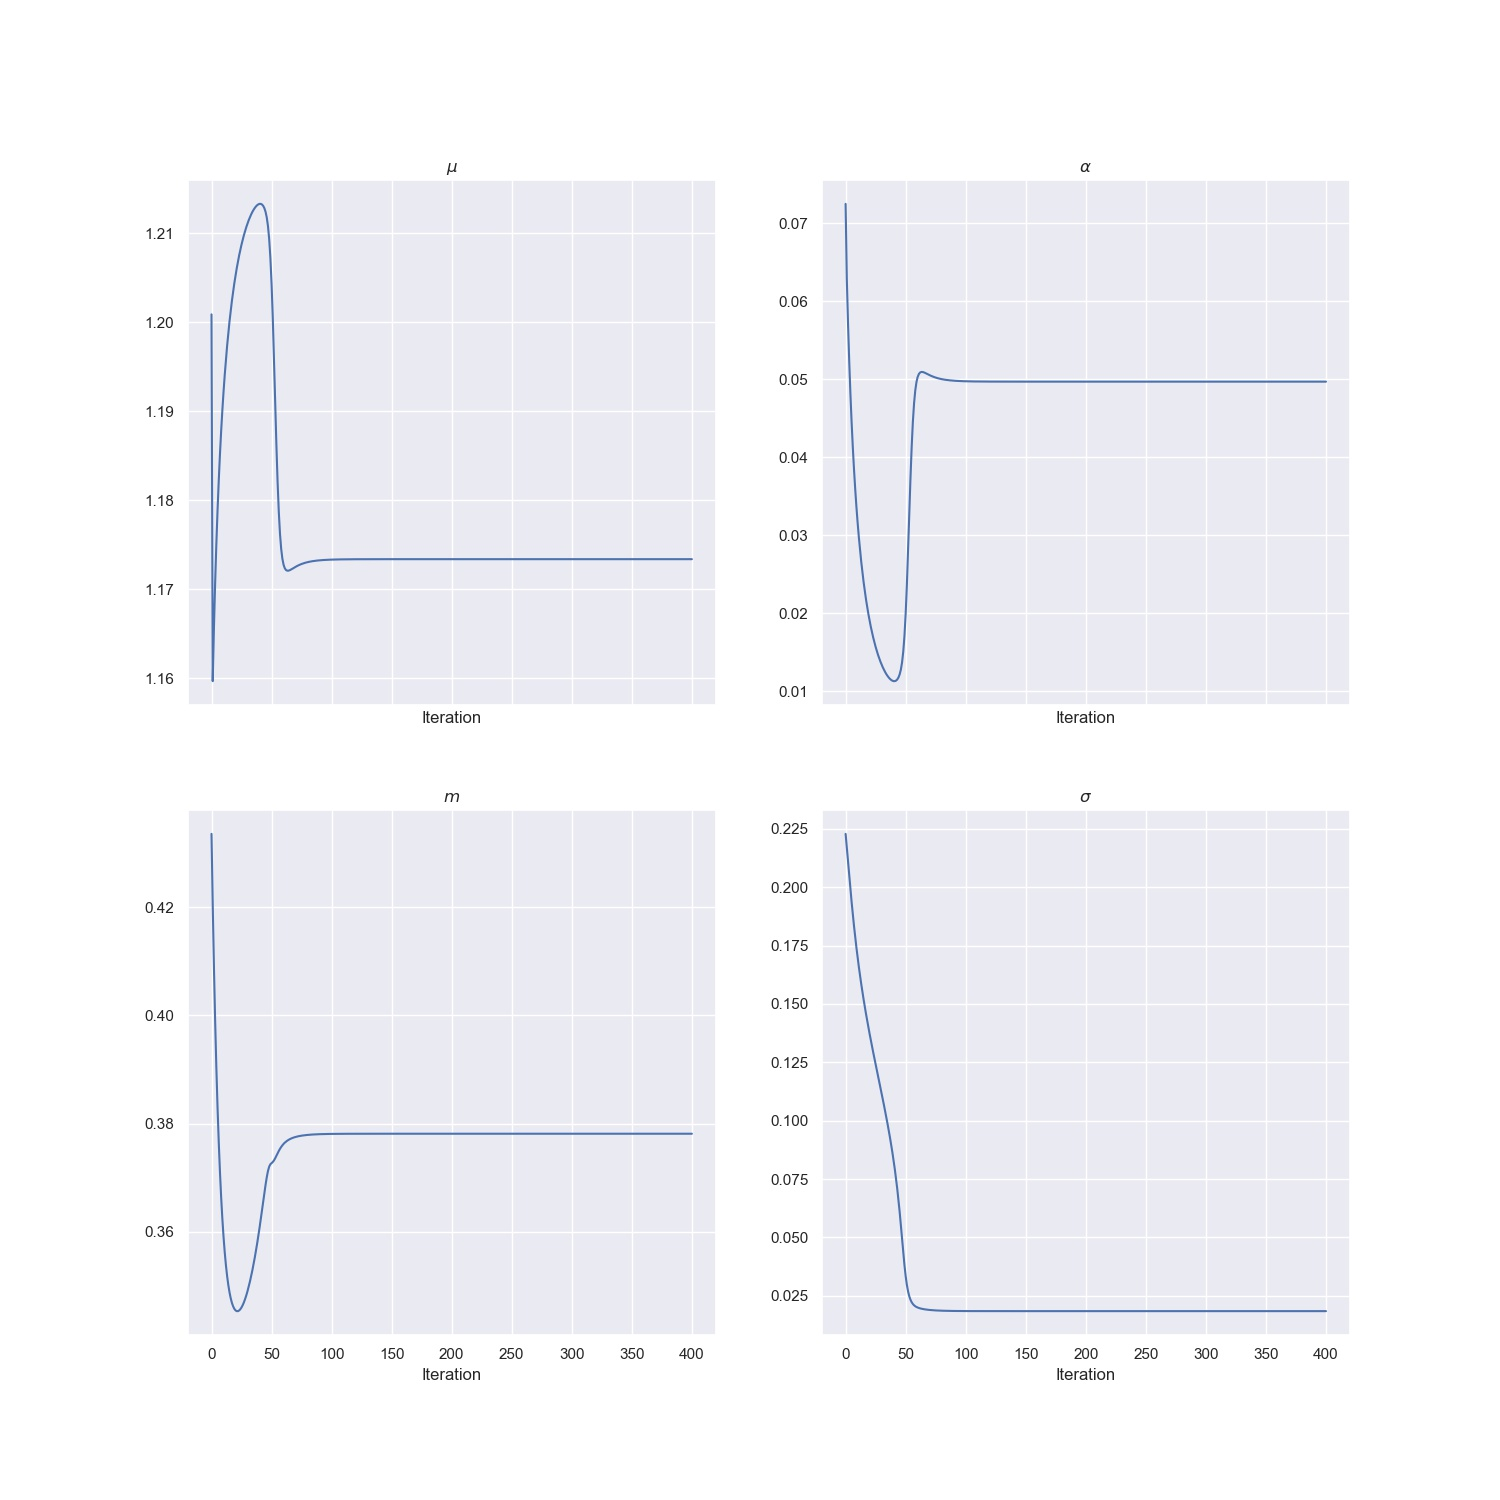
\includegraphics[width=\textwidth]{pics/results_sample/history_params_atom_0_task_1_2_3_4.jpg}
    \caption{Parameters recovery over 400 iterations with a \textit{smart} initialisation, on sample data (atom 0, task 1, 2, 3 and 4) with $\intervalleFF{a}{b} = \intervalleFF{30}{800}\times \SI{e-3}{\second}$.}
    \label{fig:history_params_atom_0_task_1_2_3_4}
\end{figure}